\documentclass[12pt]{scrartcl}

\usepackage[
  a4paper, mag=1000,
  left=2cm, right=1cm, top=2cm, bottom=2cm, headsep=0.7cm, footskip=1.27cm
]{geometry}

\usepackage[T2A]{fontenc}
\usepackage[utf8]{inputenc}
\usepackage[english,russian]{babel}
\usepackage{cmap}
\usepackage{amsmath}
\usepackage{tabularx}
\usepackage{graphicx}
\usepackage{array}
\IfFileExists{pscyr.sty}{\usepackage{pscyr}}{}
\usepackage[parfill]{parskip}
\usepackage{lastpage}
\usepackage{setspace} % single spacing between lines
\usepackage{blindtext} % for generated text - can remove
\usepackage{titlesec} % set header spacing
\usepackage{listings} %listing
\usepackage{color}
\definecolor{commentGreen}{rgb}{0,0.6,0}

\setlength{\parindent}{15pt} % paragraph indent

\lstdefinestyle{cpp}{
  language=c++,
  basicstyle=\small\ttfamily,
  breakatwhitespace=true,
  breaklines=true,
  showstringspaces=false,
  keywordstyle=\color{blue}\ttfamily,
  stringstyle=\color{red}\ttfamily,
  commentstyle=\color{commentGreen}\ttfamily,
  morecomment=[l][\color{magenta}]{\#},
  numbers=left,
  xleftmargin=1cm
}

\titlespacing{\section}{0pt}{\parskip}{-\parskip}
\titlespacing{\subsection}{0pt}{\parskip}{-\parskip}
\titlespacing{\subsubsection}{0pt}{\parskip}{-\parskip}

\usepackage[numbered]{bookmark}
\clubpenalty=10000
\widowpenalty=10000

\usepackage{fancybox,fancyhdr}
\pagestyle{fancy}
\fancyhf{}
\fancyhead[C]{\small{Олимпиадное программирование (средний уровень). Олимпиада~---~Средняя группа, 22.08.2016\\ Летняя компьютерная школа ``КЭШ'', 6--26 августа 2016 года}}

%user-defined commands

\newcommand{\inputFile}{стандартный ввод}
\newcommand{\outputFile}{стандартный вывод}

\begin{document}

\singlespacing

\section*{Задача A. Строка}

\begin{tabularx}{\textwidth}{l l X}
    Имя входного файла: & \texttt{\inputFile} \\
    Имя выходного файла: & \texttt{\outputFile} \\
    Ограничение по времени: & $1$ секунда \\
    Ограничение по памяти: & $64$ мегабайт \\
\end{tabularx}

\begin{figure}[h]
\center{
\includegraphics[width=0.5\linewidth]{A} \\}
\end{figure}

\subsection*{Формат входных данных}
На вход подается одна строка, состоящая из строчных латинских букв и цифр. Длина строки не более 256 символов.

\subsection*{Примеры}

\texttt
{
	\begin{tabularx}{0.9\textwidth}{| X | X |}
       \hline
       \multicolumn{1}{|c|}{\inputFile} & \multicolumn{1}{c|}{\outputFile} \\ 
       \hline 
       	dskjs9dks1sfd3dsa5 &
       	4 \\
       \hline
    \end{tabularx}
}

\newpage

\section*{Задача B. Безумная любовь }

\begin{tabularx}{\textwidth}{l l X}
    Имя входного файла: & \texttt{\inputFile} \\
    Имя выходного файла: & \texttt{\outputFile} \\
    Ограничение по времени: & $1$ секунда \\
    Ограничение по памяти: & $64$ мегабайт \\
\end{tabularx}

\begin{figure}[h]
\center{
\includegraphics[width=0.6\linewidth]{B} \\}
\end{figure}

Вирт, Грег, Беатрис и Конь Фред оказываются в особняке Куинси Эндикотта в поисках денег на паром. Как оказалось, Эндикотт немного не в себе из-за призрака с картины, в которого он безумно влюблен. Он хочет найти и показать эту картину братьям. На каждой картине в особняке есть подпись, но именно на портрете его возлюбленной подпись состоит только из букв $W, A, D$.

\subsection*{Формат входных данных}
На вход подаются натуральные числа $N, M (0 < N, M < 100)$~---~размеры подписи. Затем двумерный массив, описывающий подпись на картине. Он состоит из заглавных латинских букв.
\subsection*{Формат выходных данных}
Вывести ``YES'', если это та картина, и ``NO'' - если нет.


\subsection*{Примеры}

\texttt
{
	\begin{tabularx}{0.9\textwidth}{| X | X |}
       \hline
       \multicolumn{1}{|c|}{\inputFile} & \multicolumn{1}{c|}{\outputFile} \\ 
       \hline 
       \parbox[t]{\textheight}
		{       
       	3 3 \\
        WER \\
        EYR \\
        ADF \\
	   } &
	   NO \\
       \hline
    \end{tabularx}
}

\newpage

\section*{Задача C. Бендер Сгибатель Родригес }

\begin{tabularx}{\textwidth}{l l X}
    Имя входного файла: & \texttt{\inputFile} \\
    Имя выходного файла: & \texttt{\outputFile} \\
    Ограничение по времени: & $1$ секунда \\
    Ограничение по памяти: & $64$ мегабайт \\
\end{tabularx}

\begin{figure}[h]
\center{
\includegraphics[width=0.4\linewidth]{C} \\}
\end{figure}

До того, как Бендер попал в компанию ``Межпланетный экспресс'', он работал обычным роботом-сгибальщиком. Каждый день он сгибал железные балки. Каждая такая балка имела индекс, и если он был неотрицательным, то это означало, что Бендер уже ее когда-то согнул и теперь ее не нужно сгибать, иначе балку необходимо согнуть. Каждый день роботу интересно, сколько балок ему нужно согнуть.

\subsection*{Формат входных данных}
На вход подается число $N (0 < N < 100)$ - количество дней, в которые Бендер хочет знать, сколько балок нужно согнуть. Далее будут описаны N дней, то есть будет введено число $M (0 < M < 10)$ - количесвтво балок в $i$-тый день, и описание самих балок, каждый индекс балки по модулю не певосходит $100$.


\subsection*{Формат выходных данных}
Для каждого дня выяснить, сколько балок нужно согнуть. Вывести полученные значения через пробел.


\subsection*{Примеры}

\texttt
{
	\begin{tabularx}{0.9\textwidth}{| X | X |}
       \hline
       \multicolumn{1}{|c|}{\inputFile} & \multicolumn{1}{c|}{\outputFile} \\ 
       \hline 
       \parbox[t]{\textheight}
		{       
       	 	4 \\
            3 \\
            1 -2 3 \\ 
            2 \\
            1 2 \\
            4 \\
            -2 3 -4 -5 \\
	   } &
	   1 0 3 \\
       \hline
    \end{tabularx}
}

\newpage

\section*{Задача D. Даша }

\begin{tabularx}{\textwidth}{l l X}
    Имя входного файла: & \texttt{\inputFile} \\
    Имя выходного файла: & \texttt{\outputFile} \\
    Ограничение по времени: & $1$ секунда \\
    Ограничение по памяти: & $64$ мегабайт \\
\end{tabularx}

\begin{figure}[h]
\center{
\includegraphics[width=0.3\linewidth]{D} \\}
\end{figure}

Помогите Даше найти $n$-ый член последовательности: \\ 
$A[0]=A[1]=1 \\
A[2n]=A[n]+A[n-1] \\
A[2n+1]=A[n]-A[n-1] \\ $

\subsection*{Формат входных данных}
На вход подается натуральное число $n (0 < N < 40)$.

\subsection*{Формат выходных данных}
Помогите Даше найти n-ый член данной последовательности.


\subsection*{Примеры}

\texttt
{
	\begin{tabularx}{0.9\textwidth}{| X | X |}
       \hline
       \multicolumn{1}{|c|}{\inputFile} & \multicolumn{1}{c|}{\outputFile} \\ 
       \hline 
       2 &
	   2 \\
       \hline
    \end{tabularx}
}

\newpage

\section*{Задача E. Слоник и желтый мячик }

\begin{tabularx}{\textwidth}{l l X}
    Имя входного файла: & \texttt{\inputFile} \\
    Имя выходного файла: & \texttt{\outputFile} \\
    Ограничение по времени: & $1$ секунда \\
    Ограничение по памяти: & $64$ мегабайт \\
\end{tabularx}

\begin{figure}[h]
\center{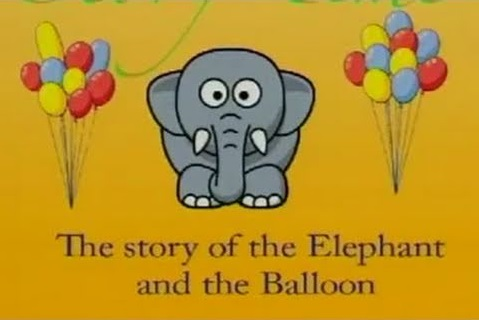
\includegraphics[width=0.4\linewidth]{E} \\}
\end{figure}

Бернард и Мэнни решили написать детскую сказку про слоника, у которого был желтый мячик. Однажды этот мячик скатился по лесенке, и Слоник очень расстроился. Для того, чтобы быстрее вернуть свой желтый мячик, Слонику необходимо найти минимальный путь через лесенку. Слоник может шагать либо на одну, либо на две ступеньки, причем на каждую $i$-ую ступеньку ему нужно затратить $A[i]$ секунд.

\subsection*{Формат входных данных}
На вход подается натуральное число $N (0 < N < 20)$~---~количество ступенек. На следующей строке описана сама лестница, т.е. $A[i]$~---~количество секунд, требуемых для преодоления $i$-ой ступеньки.
\subsection*{Формат выходных данных}
Вывести минимальное время, которое необходимо затратить Слонику для того, чтобы достать свой желтый мячик.

\subsection*{Примеры}

\texttt
{
	\begin{tabularx}{0.9\textwidth}{| X | X |}
       \hline
       \multicolumn{1}{|c|}{\inputFile} & \multicolumn{1}{c|}{\outputFile} \\ 
       \hline 
       \parbox[t]{\textheight}
		{       
       	 	2 \\
            1 2 \\
	   } &
	   	2 \\
       \hline
    \end{tabularx}
}

\newpage


\section*{Задача F. Билл Шифр }

\begin{tabularx}{\textwidth}{l l X}
    Имя входного файла: & \texttt{\inputFile} \\
    Имя выходного файла: & \texttt{\outputFile} \\
    Ограничение по времени: & $2$ секунды \\
    Ограничение по памяти: & $256$ мегабайт \\
\end{tabularx}

\begin{figure}[h]
\begin{minipage}[h]{0.3\linewidth}
\center{
\includegraphics[width=0.8\linewidth]{Bill2} \\}
\end{minipage}
\begin{minipage}[h]{0.3\linewidth}
\center{
\includegraphics[width=0.8\linewidth]{Bill} \\}
\end{minipage}
\begin{minipage}[h]{0.3\linewidth}
\center{
\includegraphics[width=0.8\linewidth]{Bill3} \\}
\end{minipage}
\end{figure}


Билл Шифр решил захватить наш мир. Для этого ему нужны могущественные союзники, но он привык ни на кого не полагаться, кроме самого себя. Поэтому после недолгих раздумий Билл пришел к выводу, что самым лучшим решением будет он сам. Так как Шифр обладает огромной силой, создание армии своих собственных клонов не составит для него никакого труда. Но вот незадача, в нашем мире магия очень нестабильна, а значит появление больших летающих треугольников может происходить лишь в строго ограниченном наборе точек пространства. Билл Шифр знает координаты всех мест, в которых может зародится один из углов его творения, но хочет узнать, какие точки будут лучшими для создания его огромных версий. Помогите Биллу узнать координаты точек, в которых получится создать наибольшего по размеру Билла Шифра (наибольший по размеру~---~имеющий наибольший периметр). 

\subsection*{Формат входных данных}
В первой строке подается число  $N$~---~количество точек для создания треугольников. Затем в каждой из $N$ строк идут координаты точек~---~$X(-1000 \leq X \leq 1000)$ и $Y(-1000 \leq Y \leq 1000)$.

\subsection*{Формат выходных данных}
Выведите координаты наибольшего треугольника. Если их несколько, то выведите любые из них. 

\subsection*{Примеры}

\texttt
{
	\begin{tabularx}{0.9\textwidth}{| X | X |}
       \hline
       \multicolumn{1}{|c|}{\inputFile} & \multicolumn{1}{c|}{\outputFile} \\ 
       \hline 
       \parbox[t]{\textheight}
       {
       3 \\
	   0 0 \\
	   1 0 \\
       0 1 \\
       } &
       \parbox[t]{\textheight}
	   {       
       0 0 \\
	   1 0 \\
       0 1 \\
	   } \\
       \hline
    \end{tabularx}
}

\newpage


\section*{Задача G. Больше, больше денег... }

\begin{tabularx}{\textwidth}{l l X}
    Имя входного файла: & \texttt{\inputFile} \\
    Имя выходного файла: & \texttt{\outputFile} \\
    Ограничение по времени: & $2$ секунды \\
    Ограничение по памяти: & $256$ мегабайт \\
\end{tabularx}

\begin{figure}[h]
\center{
\includegraphics[width=0.6\linewidth]{Stanley} \\}
\end{figure}

Стенли Пайнс владеет музеем странностей и небылиц ``Хижиной чудес''. Стен каждый месяц отладывал деньги с выручки, и в итоге за все время работы ``хижины'' накопил огромную кучу денег. Все богатство хранится в сейфе, а пароль известен только ему. После сражения с Биллом, Стенли и его брат-близнец Стенфорд решили отойти от дел и отправится в кругосветное путешествие. Для этого им, естественно, необходима большая сумма денег. Стен решил, что пришла пора воспользоваться своим накопленным добром, но вот незадача, он забыл пароль! После тщательных поисков он смог откопать бумажку, на которой был написан пароль, но в зашифрованом виде, ведь Стенли тот еще параноик. Помогите Пайнсу вернуть свои деньги, если на бумажке написан ребус: 
\begin{equation*}
	SEND + MORE = MONEY
\end{equation} 
Пароль~---~это ответ на ребус.

\subsection*{Формат входных данных}
Отсутсвует.
\subsection*{Формат выходных данных}
Выведите решение ребуса. Ребус имеет только одно решение.

\newpage

\section*{Задача H. Конфетные монстры }

\begin{tabularx}{\textwidth}{l l X}
    Имя входного файла: & \texttt{\inputFile} \\
    Имя выходного файла: & \texttt{\outputFile} \\
    Ограничение по времени: & $2$ секунды \\
    Ограничение по памяти: & $256$ мегабайт \\
\end{tabularx}

\begin{figure}[h]
\center{
\includegraphics[width=0.6\linewidth]{H} \\}
\end{figure}

Во время Хеллоуина Гравити Фолз наводнили конфетные монстры. Диппер, Мейбл и их друзья не хотят портить себе праздник, ведь они ждали его целый год, поэтому они пытаются собрать побольше сладостей и победить монстров, одновременно. Чтобы прогнать монстра необходимо отдать ему некоторое количество конфет. В результате весь вечер ребята бегали от дома к дому, собирая сладкое у старушек и отстреливаясь от чудищ конфетами. В конце вечера у них оказалось $n$ конфет. Диппер помнит, на сколько менялось количество конфет, но он совершенно забыл, как именно оно менялось каждый раз. Помогите Дипперу определить, как изменялось количество сладостей каждый раз, если в начале вечера у них не было ни одной конфеты.
\subsection*{Формат входных данных}
В первой строке находятся числа $N (2 \leq N \leq 12)$ и $S(-1000000 \leq S \leq 1000000)$, означающие количество изменений и текущее количество конфет, соотвественно. В следующей строке N чисел через пробел~---~величину каждого изменения $(0 \leq X_i \leq 50000)$
\subsection*{Формат выходных данных}
Если получить требуемый результат невозможно, вывести "No solution". Если можно, то вывести равенство. Если решение не единственное, вывести любое. Числа и знаки нужно выводить через пробел.


\subsection*{Примеры}

\texttt
{
	\begin{tabularx}{0.9\textwidth}{| X | X |}
       \hline
       \multicolumn{1}{|c|}{\inputFile} & \multicolumn{1}{c|}{\outputFile} \\ 
       \hline 
       \parbox[t]{\textheight}
		{       
       	3 10 \\
		15 25 30 \\
	   } &
	   15 + 25 - 30 = 10 \\
       \hline
       \parbox[t]{\textheight}
		{       
       	2 100 \\
		10 10 \\
	   } &
	   No solution \\
       \hline
    \end{tabularx}
}

\newpage

\end{document}
